%\addtocounter{chapter}{-1}
%\chapter[Protocolo de pruebas]{Protocolo de pruebas}
%\begin{flushright}
%\textsc{Presenta el esquema de los ensayos junto con los elementos requeridos para la toma de datos del motor.}
%\end{flushright}
\label{chap:capitulo2}
 

% Presenta el esquema propuesto para los ensayos junto con los elementos requeridos para llevar a cabo la toma de datos del motor.

 
%\vfill
\renewcommand{\mtctitle}{Protocolo de pruebas}
%\minitoc
%\newpage



\section{Capitulo 2: Caracterización del caso de estudio en Industria 4.0}

Este capítulo presenta la caracterización del caso de estudio correspondiente a un proyecto de integración IIoT desarrollado por DAUTOM S.A.S. en el sector de la molinería. Se describe en detalle el área de empaque, su flujo operacional, la infraestructura IIoT implementada y los principales requerimientos y desafíos identificados en materia de analítica de datos.


\subsection{\centering Descripción del caso de estudio}

El caso de estudio se centra en un proyecto desarrollado por DAUTOM S.A.S., empresa santandereana con experiencia en integración de soluciones IIoT y Smart Manufacturing, con implementaciones destacadas en el sector de la molinería. En Barranquilla, se ejecutó un proyecto de integración IIoT que incorporó a la plataforma industrial diferentes áreas de producción, entre las cuales se encuentra el área de empacadoras de harina, encargada de envasar la harina para su comercialización.\\


La información recolectada se emplea para calcular rendimientos de proceso, evaluar la disponibilidad de máquinas y controlar la calidad. Todos los datos se centralizan en una arquitectura Unified Namespace (UNS), lo que habilita una única fuente de verdad, reduce silos de información y facilita el despliegue de analítica avanzada.\\


\subsubsection{\centering Área de Empacadoras}

El área de empacadoras es la encargada de tomar la harina producida en los molinos y envasarla en presentaciones de libra y kilo, listas para su posterior comercialización. Esta área representa el punto final de la cadena de producción antes de la distribución al cliente.

En este proyecto se integraron dos áreas de empaque diferenciadas, cada una especializada en el procesamiento de diferentes tipos de harina:

\begin{itemize}
    \item \textbf{Empaque de Trigo:} Dedicada al envasado de harina de trigo en presentaciones de libra y kilo.
    \item \textbf{Empaque de Maíz:} Dedicada al envasado de harina de maíz en presentaciones de libra y kilo.
\end{itemize}

Cada área cuenta con dos líneas de producción independientes, conformadas por los siguientes elementos principales:

\subsubsection{Componentes de la línea de producción de empaque}

Cada línea de producción en el área de empacadoras está compuesta por los siguientes equipos:

\begin{enumerate}
    \item \textbf{Empacadoras:} Máquinas encargadas de envasar la harina en bolsas de una libra o de un kilo. Cada línea de producción dispone de dos empacadoras, lo que permite mantener la continuidad operativa en caso de mantenimiento o fallas en una de ellas.
    
    \item \textbf{Enfardadora:} Equipo encargado de agrupar las bolsas ya empacadas en fardos de mayor tamaño para facilitar su manejo, almacenamiento y transporte. La configuración de cada fardo varía según la presentación:
    \begin{itemize}
        \item Para la referencia de libra: cada fardo contiene 24 unidades.
        \item Para la referencia de kilo: cada fardo contiene 20 unidades.
    \end{itemize}
\end{enumerate}

Los fardos resultantes se apilan en estibas para su almacenamiento temporal o despacho directo al cliente final, completando así el ciclo productivo.

\subsection{Flujo operacional y fuentes de datos}

El flujo de producción del área de empaque inicia una vez que la harina procesada en los molinos es almacenada en silos intermedios. A partir de este punto, se ejecutan las siguientes etapas operacionales:

\subsubsection{Descripción del flujo operacional}

\begin{enumerate}
    \item \textbf{Almacenamiento intermedio:} La harina proveniente de los molinos de trigo y maíz se dirige a silos de almacenamiento de harina, que cumplen la función de regular el suministro hacia las áreas de empaque. Es importante señalar que esta etapa no se encuentra integrada en la red IIoT del proyecto, por lo que no se dispone de telemetría ni datos en tiempo real de los niveles de los silos.
    
    \item \textbf{Área de empaque:} Desde los silos de harina, el producto se traslada mediante sistemas de transporte neumático y mecánico hacia el área de empacadoras. En esta etapa:
    \begin{itemize}
        \item La harina es dosificada y envasada en presentaciones de 1 libra y 1 kilogramo mediante las empacadoras.
        \item Las bolsas individuales son agrupadas y embaladas en fardos mediante las enfardadoras.
        \item Los fardos se apilan en estibas para su almacenamiento y posterior distribución al cliente final.
    \end{itemize}
\end{enumerate}

\subsubsection{Fuentes de datos disponibles}

La infraestructura de adquisición de datos del área de empaque se basa en una arquitectura distribuida de controladores industriales que capturan información operativa en tiempo real. A continuación se describen las fuentes de datos y la información que proporcionan.

\subsubsection{Arquitectura de control y adquisición de datos}

Cada área de empaque (Trigo y Maíz) cuenta con dos líneas de producción independientes. Por línea se tienen:

\begin{itemize}
    \item 2 empacadoras
    \item 1 enfardadora
\end{itemize}

Lo que resulta en un total de \textbf{4 empacadoras y 2 enfardadoras por área de empaque}.

La jerarquía de control se estructura de la siguiente manera:

\paragraph{PLCs de empacadoras (Omron)}
Cada empacadora cuenta con un PLC Omron dedicado que gestiona su lógica de control y captura las siguientes variables de proceso:

\begin{itemize}
    \item \textbf{Conteo de bolsas producidas:} Contador acumulado de unidades empacadas
    \item \textbf{Tiempo de ciclo:} Tiempo requerido para completar el empaque de una unidad
    \item \textbf{Estado actual de la máquina:} Estado operativo (marcha, paro, alarma, mantenimiento)
\end{itemize}

Dado que cada área tiene 4 empacadoras, se cuenta con un total de \textbf{4 PLCs Omron por área de empaque}.

\paragraph{Señales I/O de enfardadoras}
Las enfardadoras cuentan con PLCs dedicados pero unicamente tenemos acceso a sñales de entrada/salida (I/O) que proporcionan la siguiente información:

\begin{itemize}
    \item \textbf{Conteo de bolsas entrantes:} Señal de pulsos que cuenta las bolsas que ingresan a la enfardadora
    \item \textbf{Estado de actividad:} Señal digital que indica si la enfardadora está activa o inactiva
    \item \textbf{Conteo de fardos producidos:} Contador de fardos completos generados
\end{itemize}

\paragraph{PLC de recolección de datos (Weidmüller)}
Cada área de empaque cuenta con un PLC Weidmüller que actúa como concentrador de datos. Este dispositivo cumple las siguientes funciones:

\begin{itemize}
    \item Recopila información de los 4 PLCs Omron de las empacadoras mediante comunicación industrial
    \item Adquiere las señales I/O de las 2 enfardadoras
    \item Normaliza y estructura los datos según un formato estándar
    \item Comunica con el centro de datos mediante protocolo OPC UA
    \item Actúa como Edge Gateway hacia la arquitectura UNS
\end{itemize}

\subsubsection{Resumen de variables importantes monitorizadas}

La Tabla \ref{tab:variables_monitorizadas} resume las variables capturadas por tipo de equipo y su uso en la analítica de producción.

\begin{table}[H]
\centering
\caption{Variables monitorizadas por tipo de equipo}
\label{tab:variables_monitorizadas}
\begin{tabular}{|l|l|p{6cm}|}
\hline
\textbf{Equipo} & \textbf{Variable} & \textbf{Uso en analítica} \\
\hline
\multirow{4}{*}{\textbf{Empacadora}} & Conteo de bolsas & Cálculo de producción total, rendimiento, OEE \\
\cline{2-3}
& Tiempo de ciclo & Análisis de eficiencia, detección de degradación \\
\cline{2-3}
& Estado de máquina & Cálculo de disponibilidad, análisis de paros \\
\hline
\multirow{2}{*}{\textbf{Enfardadora}} & Conteo de bolsas & Validación de flujo de producción \\
\cline{2-3}
& Estado de actividad & Cálculo de disponibilidad \\
\cline{2-3}
& Conteo de fardos & Cálculo de producción final, inventario \\
\hline
\end{tabular}
\end{table}

Todos estos datos se transmiten desde los PLCs Weidmüller hacia el centro de datos mediante el protocolo OPC UA, donde son integrados en la arquitectura UNS de la plataforma Ignition.

\subsection{Arquitectura de la infraestructura IIoT}

La infraestructura IIoT implementada en el proyecto sigue una arquitectura basada en el concepto de Unified Namespace (UNS), donde todos los datos de las diferentes fuentes se centralizan en un unico espacio. Esta arquitectura se representa en la Figura \ref{fig:arquitectura_iiot}.

\begin{figure}[H]
    \centering
    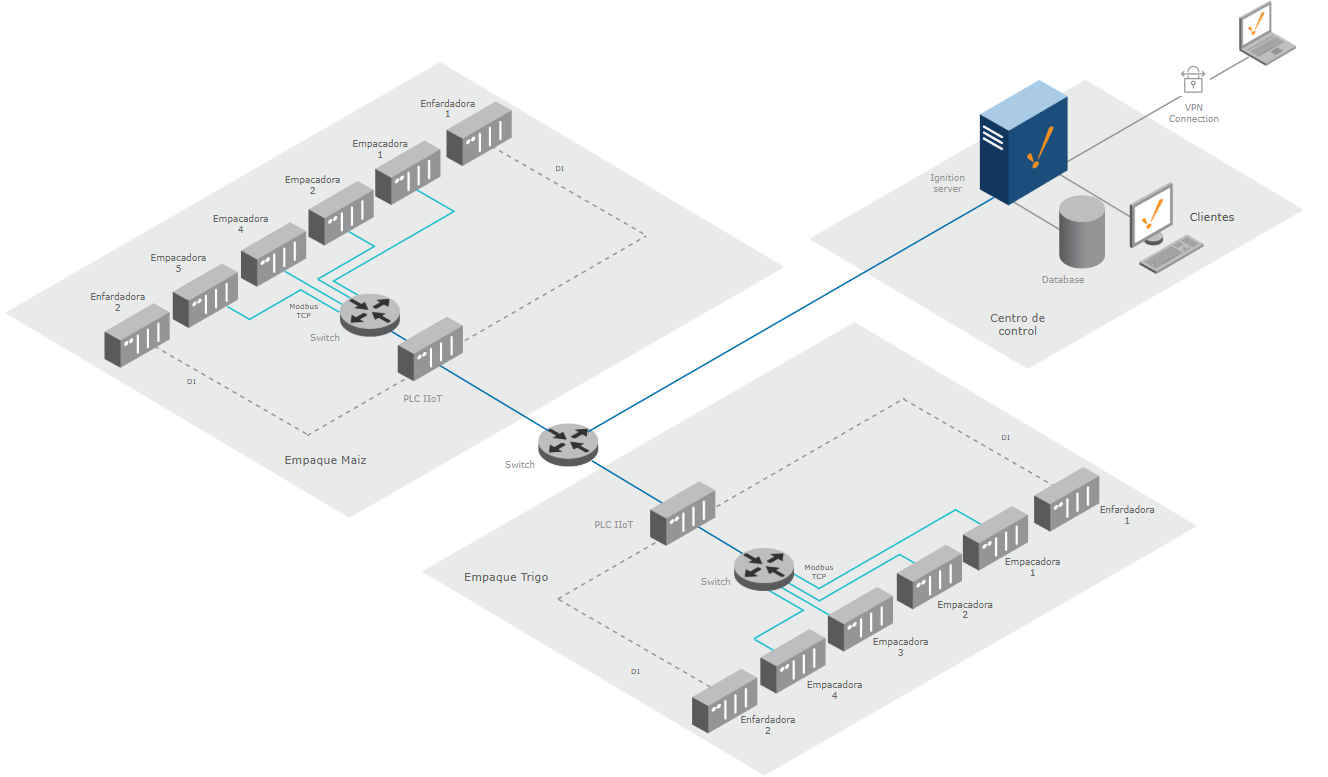
\includegraphics[width=1\textwidth]{Figuras/diagrama_arquitectura.png}
    \caption{Arquitectura IIoT del sistema de empaque integrado con UNS}
    \label{fig:arquitectura_iiot}
\end{figure}

\subsubsection{Componentes de la arquitectura}

La arquitectura IIoT implementada se compone de las siguientes capas y componentes:

\subsubsection{Capa de dispositivos de campo}

Esta capa incluye todos los controladores y señales que interactúan directamente con los procesos físicos de producción:

\begin{itemize}
    \item \textbf{PLCs Omron (8 unidades total):} 4 PLCs por área de empaque (1 por cada empacadora), encargados del control local y captura de variables de proceso.
    
    \item \textbf{Señales I/O de enfardadoras (4 unidades total):} 2 conjuntos de señales por área, que monitorizan el estado y conteo de las enfardadoras.
\end{itemize}

\subsubsection{Capa Edge/Gateway}

En esta capa se encuentran los PLCs Weidmüller que actúan como concentradores de datos (Data Gateways) para cada área de empaque:

\begin{itemize}
    \item \textbf{PLC Weidmüller - Área Empaque Trigo:} Recopila datos de las 4 empacadoras (PLCs Omron) y las 2 enfardadoras (señales I/O) del área de trigo.
    
    \item \textbf{PLC Weidmüller - Área Empaque Maíz:} Recopila datos de las 4 empacadoras (PLCs Omron) y las 2 enfardadoras (señales I/O) del área de maíz.
\end{itemize}

Las funciones principales de estos dispositivos incluyen:

\begin{itemize}
    \item Adquisición de datos desde PLCs Omron mediante protocolos industriales estándar
    \item Captura de señales I/O digitales de las enfardadoras
    \item Normalización y estructuración de datos en un formato unificado
    \item Comunicación con el centro de datos mediante protocolo OPC UA
    \item Buffering local de datos para garantizar entrega confiable ante fallas de red
\end{itemize}

\subsubsection{Capa de comunicación - OPC UA}

El protocolo OPC UA (Open Platform Communications Unified Architecture) se utiliza como medio de comunicación entre los PLCs Weidmüller y el centro de datos. Este protocolo industrial ofrece:

\begin{itemize}
    \item \textbf{Interoperabilidad:} Estándar abierto compatible con múltiples plataformas y fabricantes
    \item \textbf{Seguridad:} Cifrado de comunicaciones y autenticación de dispositivos
    \item \textbf{Orientación a objetos:} Modelado de información que facilita la organización jerárquica
\end{itemize}

\subsubsection{Capa UNS (Unified Namespace) - Centro de datos}

El núcleo de la arquitectura reside en el centro de datos, donde se implementa el Unified Namespace mediante la plataforma Ignition. Los componentes clave son:

\paragraph{Ignition Gateway}
Servidor central que:
\begin{itemize}
    \item Establece conexiones OPC UA con los PLCs Weidmüller de cada área
    \item Adquiere datos en tiempo real de todas las variables de proceso
    \item Aloja la aplicación MES (Manufacturing Execution System) para el agendamiento y gestión de órdenes de producción del área de empaque
\end{itemize}

La aplicación MES implementada en Ignition permite:
\begin{itemize}
    \item Crear y gestionar órdenes de producción para cada línea de empaque (Trigo y Maíz)
    \item Agendar la producción según demanda, disponibilidad de materia prima y capacidad de las líneas
    \item Asignar productos, cantidades objetivo y tiempos estimados a cada orden
    \item Hacer seguimiento en tiempo real del avance de cada orden de producción
    \item Registrar eventos de inicio, pausa y finalización de órdenes
    \item Asociar los datos de producción capturados (conteo de bolsas, tiempos, estados) con las órdenes activas
\end{itemize}

La integración entre el MES y los datos en tiempo real del UNS habilita el cálculo automático de KPIs operacionales, tales como:
\begin{itemize}
    \item \textbf{OEE (Overall Equipment Effectiveness):} Calculado a partir de la disponibilidad, rendimiento y calidad de cada empacadora en relación con las órdenes programadas
    \item \textbf{Cumplimiento de órdenes:} Porcentaje de órdenes completadas dentro del tiempo estimado
    \item \textbf{Eficiencia de línea:} Relación entre producción real y producción planificada por línea
    \item \textbf{Tiempo de ciclo promedio:} Promedio de tiempo requerido para empacar una unidad durante la orden
    \item \textbf{Tasa de producción:} Unidades producidas por hora en cada línea
    \item \textbf{Utilización de equipos:} Porcentaje del tiempo que cada empacadora estuvo activa durante el turno
\end{itemize}

Esta integración MES-UNS elimina la necesidad de captura manual de datos de producción y garantiza que todos los KPIs se basen en información confiable y en tiempo real.

\paragraph{Base de datos histórica}
Almacena series temporales de todas las variables para:
\begin{itemize}
    \item Análisis retrospectivo de producción
    \item Cumplimiento de requisitos de trazabilidad
\end{itemize}


\subsection{Estructura del namespace}

El namespace se estructura siguiendo una jerarquía basada en el estándar ISA-95, organizando los datos de forma lógica desde el nivel de empresa hasta el nivel de dispositivo individual. La estructura implementada para el caso de estudio es la siguiente:

\begin{verbatim}
Empresa/
└── Planta_Barranquilla/
    ├── Area_Empaque_Trigo/
    │   ├── Linea_1/
    │   │   ├── Empacadora_1/
    │   │   │   ├── Conteo_Bolsas
    │   │   │   ├── Tiempo_Ciclo
    │   │   │   ├── Estado_Maquina
    │   │   │   └── Eventos
    │   │   ├── Empacadora_2/
    │   │   │   ├── Conteo_Bolsas
    │   │   │   ├── Tiempo_Ciclo
    │   │   │   ├── Estado_Maquina
    │   │   │   └── Eventos
    │   │   └── Enfardadora/
    │   │       ├── Conteo_Bolsas_Entrada
    │   │       ├── Estado_Actividad
    │   │       └── Conteo_Fardos
    │   ├── Linea_2/
    │   │   ├── Empacadora_1/
    │   │   ├── Empacadora_2/
    │   │   └── Enfardadora/
    │   └── KPIs_Area/
    │       ├── Produccion_Total
    │       ├── OEE_Promedio
    │       └── Disponibilidad
    └── Area_Empaque_Maiz/
        ├── Linea_1/
        │   ├── Empacadora_1/
        │   ├── Empacadora_2/
        │   └── Enfardadora/
        ├── Linea_2/
        │   ├── Empacadora_1/
        │   ├── Empacadora_2/
        │   └── Enfardadora/
        └── KPIs_Area/
            ├── Produccion_Total
            ├── OEE_Promedio
            └── Disponibilidad
\end{verbatim}

\subsubsection{Niveles de la jerarquía}

La estructura del namespace sigue los siguientes niveles jerárquicos:

\paragraph{Nivel 1 - Empresa}
Nodo raíz que agrupa todas las instalaciones de la organización.

\paragraph{Nivel 2 - Planta/Sitio}
Identifica la ubicación física de la instalación (en este caso, Planta\_Barranquilla).

\paragraph{Nivel 3 - Área}
Agrupa los equipos por área funcional de producción:
\begin{itemize}
    \item Area\_Empaque\_Trigo
    \item Area\_Empaque\_Maiz
\end{itemize}

\paragraph{Nivel 4 - Línea de producción}
Cada área cuenta con dos líneas de producción independientes (Linea\_1, Linea\_2).

\paragraph{Nivel 5 - Equipo}
Identifica cada equipo individual dentro de la línea:
\begin{itemize}
    \item Empacadora\_1, Empacadora\_2 (por línea)
    \item Enfardadora (por línea)
\end{itemize}

\paragraph{Nivel 6 - Variables de proceso}
Tags individuales que contienen los valores de las variables monitorizadas.

\subsubsection{Ejemplo de rutas completas de tags}

A continuación se muestran ejemplos de rutas completas para algunos tags del sistema:

\begin{verbatim}
Empresa/Planta_Barranquilla/Area_Empaque_Trigo/Linea_1/
    Empacadora_1/Conteo_Bolsas

Empresa/Planta_Barranquilla/Area_Empaque_Maiz/Linea_2/
    Enfardadora/Estado_Actividad

Empresa/Planta_Barranquilla/Area_Empaque_Trigo/KPIs_Area/
    OEE_Promedio
\end{verbatim}

Esta nomenclatura garantiza que cualquier aplicación o usuario pueda identificar unívocamente la procedencia y significado de cada dato en el sistema.

\subsection{Requerimientos y desafíos de analítica de datos}

A partir de reuniones técnicas realizadas con el tutor designado por DAUTOM S.A.S., quien proporcionó acompañamiento especializado durante la caracterización del caso de estudio, se identificaron los requerimientos clave para la integración de una herramienta basada en LLM a la arquitectura UNS existente. Estas sesiones de trabajo permitieron comprender en profundidad las necesidades operacionales de la planta, los puntos críticos en la toma de decisiones y las limitaciones actuales en el acceso y análisis de información. 

A continuación se presentan los tres requerimientos principales identificados, junto con los desafíos técnicos asociados a cada uno de ellos. 

\subsubsection{Análisis detallado de requerimientos y desafíos}

A continuación se describe en detalle cada requerimiento identificado y los desafíos técnicos asociados a su implementación.

\paragraph{Requerimiento 1: Interpretación de consultas en lenguaje natural con conocimiento técnico del dominio}

\textbf{Descripción del requerimiento:}

El sistema LLM debe comprender consultas en lenguaje natural que incluyan términos técnicos de manufactura y ser capaz de identificar qué datos del UNS necesita consultar para responder. Esto implica que usuarios sin conocimientos técnicos profundos puedan realizar preguntas complejas sobre el proceso productivo y obtener respuestas precisas y contextualizadas.

\textbf{Desafíos identificados:}

\textit{D1.1 - Ambigüedad en términos técnicos:}

Palabras como "disponibilidad", "rendimiento" o "producción" pueden tener diferentes significados según el contexto en el que se utilicen. Por ejemplo, "disponibilidad" puede referirse a si la máquina está funcionando (uptime) o a si hay material disponible para producir. Similarmente, "rendimiento" puede aludir al rendimiento de una máquina individual (unidades producidas por hora) o al rendimiento global de una línea de producción.

El LLM debe entender el contexto de la pregunta para interpretar correctamente el término y acceder a las variables apropiadas del namespace. Esto requiere no solo procesamiento de lenguaje natural, sino también conocimiento del dominio industrial y la semántica de las métricas de manufactura.

\textit{D1.2 - Comprensión de relaciones entre variables:}

Preguntas como "¿por qué bajó la producción ayer?" requieren analizar múltiples factores que pueden estar relacionados: paros de máquinas no programados, incremento en tiempos de ciclo, cambios de producto que requieren ajustes, o falta de material en los silos. El LLM debe saber qué variables están relacionadas causalmente y buscar correlaciones entre ellas, no solo reportar un dato aislado.

Este desafío implica que el modelo debe tener capacidad de razonamiento sobre las relaciones funcionales entre diferentes componentes del sistema productivo y cómo estas interacciones afectan los KPIs resultantes.

\textit{D1.3 - Mapeo de lenguaje natural a la estructura del namespace:}

El usuario puede utilizar referencias ambiguas como "la empacadora de trigo" sin especificar cuál de las 4 empacadoras del área de trigo se está consultando. De manera similar, expresiones como "la línea A" pueden referirse a Línea A de Trigo o Línea A de Maíz.

El LLM debe ser capaz de pedir aclaraciones cuando sea necesario ("¿Te refieres a la Línea 1 del área de Trigo o de Maíz?") o usar el contexto previo de la conversación para resolver la ambigüedad de forma inteligente. Esto requiere mantener estado conversacional y aplicar heurísticas de resolución de referencias.

\paragraph{Requerimiento 2: Generación de reportes personalizados con análisis comparativos}

\textbf{Descripción del requerimiento:}

La herramienta debe generar reportes que no solo muestren números crudos, sino que incluyan comparaciones útiles (vs. día anterior, vs. otras líneas, vs. meta establecida en la orden de producción) y detecten automáticamente anomalías o patrones relevantes para la toma de decisiones.

\textbf{Desafíos identificados:}

\textit{D2.1 - Identificar qué comparaciones son relevantes:}

No todas las comparaciones tienen sentido o aportan valor en el contexto de manufactura. Por ejemplo, comparar la producción de un lunes con un domingo puede ser engañoso si los turnos de fin de semana operan con menor personal o producen referencias diferentes.

El LLM debe incorporar lógica operacional para saber qué comparaciones aportan valor en cada contexto. Esto incluye comparaciones con el mismo día de la semana anterior (para eliminar efectos de calendario), comparaciones entre líneas que producen el mismo producto (para identificar ineficiencias relativas), y comparaciones contra las metas establecidas en las órdenes de producción del MES.

\textit{D2.2 - Combinar datos de múltiples fuentes:}

Para generar reportes completos y contextualizados, el LLM debe integrar información de tres fuentes principales:

\begin{itemize}
    \item \textbf{UNS:} Datos operacionales en tiempo real (conteos actuales de bolsas, tiempos de ciclo recientes, estados actuales de máquinas, eventos de alarma activos).
    
    \item \textbf{MES integrado en Ignition:} Información contextual sobre la operación (qué orden de producción está activa, qué producto se está empacando, cantidades objetivo planificadas, tiempos programados de inicio y fin).
    
    \item \textbf{Base de datos histórica:} Datos de producción de días, semanas o meses anteriores que permiten análisis de tendencias, detección de degradación de equipos, y comparaciones temporales.
\end{itemize}

La integración coherente de estas fuentes permite que el LLM genere análisis completos. Por ejemplo: "La producción de hoy está 15\% por debajo del mismo día de la semana pasada (BD histórica), la Línea 1 está trabajando en la Orden \#12345 de harina de trigo presentación kilo con una meta de 5000 unidades (MES), y actualmente la Empacadora 2 está en estado de alarma desde hace 10 minutos (UNS), lo que explica la desviación observada".

Este desafío requiere que el LLM orqueste consultas a múltiples sistemas, reconcilie diferencias en granularidad temporal entre fuentes, y sintetice la información de forma coherente.

\textit{D2.3 - Adaptar el reporte según el perfil del usuario:}

Diferentes stakeholders en la organización tienen necesidades de información distintas:

\begin{itemize}
    \item Un \textbf{gerente de producción} necesita ver KPIs agregados por área, tendencias semanales o mensuales, y comparaciones de eficiencia entre turnos o líneas.
    
    \item Un \textbf{supervisor de turno} necesita detalles específicos sobre qué ocurrió durante su periodo de responsabilidad, en qué equipos se presentaron problemas, y qué acciones correctivas se tomaron.
    
    \item Un \textbf{técnico de mantenimiento} necesita información sobre frecuencia de fallas por equipo, tiempos promedio de reparación, y patrones de degradación que sugieran mantenimientos preventivos.
\end{itemize}

El sistema debe ser capaz de ajustar automáticamente el contenido, nivel de detalle, métricas presentadas y formato de salida según el perfil del usuario que realiza la consulta. Esto implica implementar perfiles de usuario con permisos y preferencias diferenciadas.

\paragraph{Requerimiento 3: Acceso eficiente a datos históricos y en tiempo real}

\textbf{Descripción del requerimiento:}

El sistema debe poder consultar tanto los datos en tiempo real disponibles en el UNS como el histórico almacenado en bases de datos relacionales, y combinarlos de forma coherente para responder consultas que abarquen diferentes periodos de tiempo, desde minutos recientes hasta meses o años anteriores.

\textbf{Desafíos identificados:}

\textit{D3.1 - Generar consultas eficientes a la base de datos:}

El LLM debe traducir preguntas en lenguaje natural a consultas de base de datos (SQL) que sean eficientes y no generen carga computacional excesiva. Por ejemplo, si el usuario pregunta "¿cuál fue el promedio de producción del último mes?", el LLM debe generar una query que utilice tablas agregadas pre-calculadas o índices apropiados, en lugar de escanear millones de registros individuales.

Esto requiere que el LLM tenga conocimiento de:
\begin{itemize}
    \item El esquema de la base de datos (tablas, columnas, relaciones)
    \item Los índices disponibles y cómo aprovecharlos
    \item Estrategias de agregación eficiente (uso de tablas materializadas, vistas agregadas)
    \item Limitaciones de rendimiento del sistema de base de datos
\end{itemize}

La generación de queries SQL eficientes es crítica para garantizar tiempos de respuesta aceptables, especialmente cuando se consultan periodos extensos con alta densidad de datos.

\textit{D3.2 - Seleccionar la granularidad adecuada de los datos:}

Los datos industriales se almacenan con diferentes frecuencias de muestreo dependiendo de la variable y el propósito. Para periodos cortos de tiempo (última hora, último turno) es apropiado usar datos de alta frecuencia que capturan cada evento significativo. Sin embargo, para periodos largos (último mes, último trimestre) es más eficiente usar agregaciones por hora, por turno, o por día.

El LLM debe decidir automáticamente qué nivel de detalle (granularidad) usar según el rango temporal que especifica el usuario en su consulta. Por ejemplo:
\begin{itemize}
    \item "Producción en los últimos 30 minutos" → datos con granularidad de minutos
    \item "Producción del día de ayer" → datos agregados por hora
    \item "Producción del último mes" → datos agregados por día o por turno
\end{itemize}

Esta selección automática de granularidad balancea la precisión de la respuesta con la eficiencia computacional, evitando procesar datos innecesariamente detallados cuando no aportan valor adicional a la consulta.

\subsubsection{Síntesis de requerimientos y desafíos}

Los tres requerimientos identificados y sus desafíos asociados representan los aspectos técnicos críticos que debe abordar la integración de una herramienta LLM con la arquitectura UNS del caso de estudio. El Requerimiento 1 se enfoca en las capacidades de comprensión del lenguaje natural y mapeo al dominio industrial. El Requerimiento 2 aborda la generación inteligente de insights y la personalización de reportes. El Requerimiento 3 trata los aspectos de arquitectura de datos y eficiencia en el acceso a información histórica y en tiempo real.

Estos requerimientos guiarán el diseño de la solución propuesta en los capítulos subsiguientes y servirán como base para la definición de métricas de validación del sistema integrado.




